\documentclass[10pt,a4paper]{article}
\usepackage[utf8]{inputenc}
\usepackage[spanish]{babel}
\usepackage{amsmath}
\usepackage{amsfonts}
\usepackage{amssymb}
\usepackage{graphicx}
\usepackage[left=2cm,right=2cm,top=2cm,bottom=2cm]{geometry}
\usepackage[hidelinks]{hyperref}
\usepackage{listings}
\lstset{
    frame = single,     
	framexleftmargin = 15pt
}

\begin{document}

\begin{titlepage}
\title{\textbf{{\Huge Práctica 2 - Sistemas Legados}}}
\author{
	Pedro Allué Tamargo (758267)
	\and
	Juan José Tambo Tambo (755742)
	\and
	Jesús Villacampa Sagaste (755739)
}
\clearpage\maketitle
\thispagestyle{empty}
\tableofcontents
\end{titlepage}

\section{Esfuerzos invertidos}

\begin{itemize}
\item Pedro Allué Tamargo:
\item Juan José Tambo Tambo:
\item Jesús Villacampa Sagaste:
\end{itemize}

\section{Instalación del emulador}

Para la realización de esta práctica se ha utilizado el Sistema Operativo \emph{Ubuntu}. Para instalar el emulador \emph{x3270}\footnote{\url{http://x3270.bgp.nu/}} se ejecutarán las órdenes:

\begin{lstlisting}
sudo apt update
sudo apt -y install x3270
\end{lstlisting}

Estas instrucciones instalarán el emulador y las herramientas de \emph{scrapping} (\emph{s3270}).\\

Para conectar el \emph{scrapper} con el \emph{mainframe} se ejecutará la orden:

\begin{lstlisting}
s3270 155.210.152.51:101
\end{lstlisting}


\section{Descripción de la aplicación legada}

La aplicación legada se corresponde con una lista de tareas. El usuario podrá añadir dos tipos distintos de tareas: tareas generales y tareas específicas.\\
Esta distinción implica que las tareas específicas disponen de un campo ``nombre'' del que no disponen las generales.\\
Otro punto a tener en cuenta de la aplicación legada es que las tareas guardadas durante una ejecución no son persistentes. Es decir, las tareas no se conservan de una ejecución a otra.\\
Al realizar la comunicación con la aplicación, han aparecido una serie de problemas con el número máximo de carácteres que se admiten a la hora de asignar nuevas tareas. En las tareas generales, si se considera que se introducen 4 dígitos en la fecha, admite 12 como máximo para la descripción. En cuanto a las específicas, 
\newpage
\section{Implementación del Wrapper}

Se pide realizar una aplicación con interfaz gráfica que encapsule el acceso a la aplicación legada. Se ha elegido \emph{Java} como lenguaje para implementar este \emph{wrapper}.

\subsection{Modelo de datos}

El modelo de datos se compone de 2 clases (Figura \ref{fig:tasks_class_diagram}) que representan las distintas estructuras de datos que son las tareas de la aplicación legada.

\begin{figure}[h!]
\centering
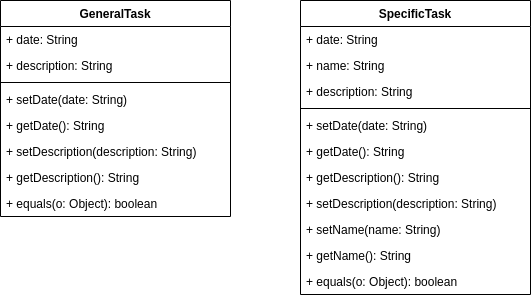
\includegraphics[scale=0.5]{images/class_diagram.png}
\caption{Diagrama de clases UML de Tareas}
\label{fig:tasks_class_diagram}
\end{figure}

Las clases se componen de los mismos elementos que la aplicación legada. En el caso de \emph{GeneralTask} se compone de 2 campos: fecha y descripción. En el caso de \emph{SpecificTask} se compone de 3 campos: fecha, nombre y descripción.

\subsection{Interfaz gráfica de usuario}

La interfaz gráfica de usuario (GUI) se basa en las librerías gráficas \emph{javax.swing} y \emph{java.awt}.\\
Se ha estructurado la aplicación de tal manera que el usuario al iniciarla puede elegir entre acceder a las tareas generales o a las específicas (Figura \ref{fig:main_screen}).

\begin{figure}[h!]
\centering
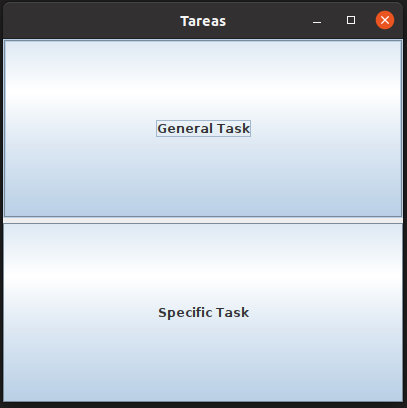
\includegraphics[scale=0.4]{images/main_screen.png}
\caption{Pantalla principal de la aplicación}
\label{fig:main_screen}
\end{figure}

Tras acceder a la opción de \emph{General Task} se puede observar una tabla que muestra las distintas tareas del tipo ``General'' que se han introducido en la aplicación (Figura \ref{fig:general_task_screen}).

\newpage
\begin{figure}[h!]
\centering
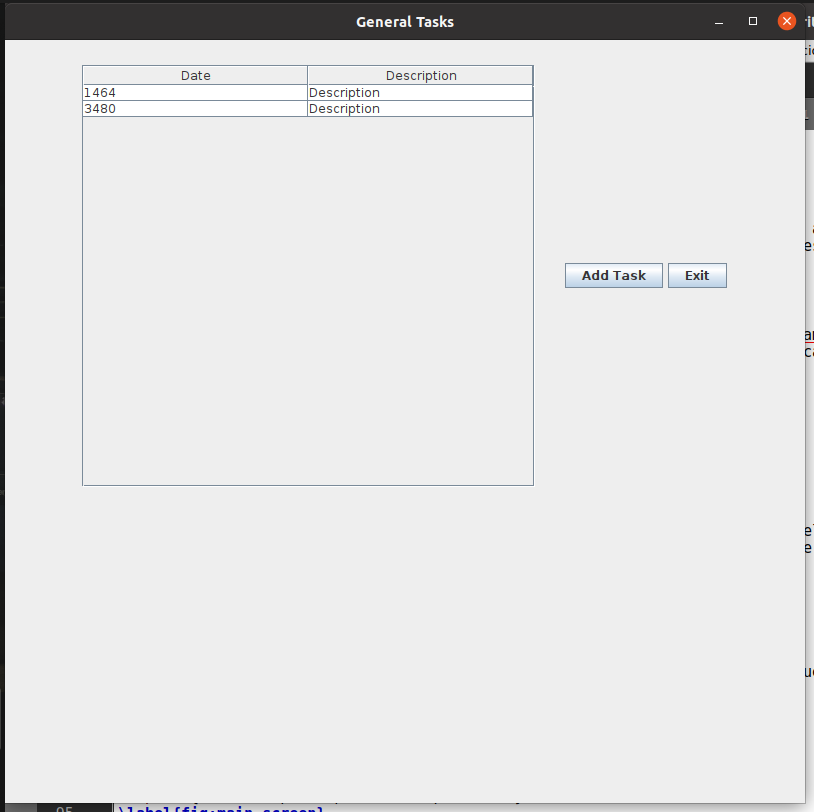
\includegraphics[scale=0.4]{images/general_task_screen.png}
\caption{Pantalla que muestra las tareas generales de la aplicación}
\label{fig:general_task_screen}
\end{figure}

Si en esta pantalla se pulsa sobre el botón \emph{``Add Task''} se abrirá una nueva ventana donde podremos introducir una nueva tarea a la aplicación (Figura \ref{fig:add_general_task_screen}).

\begin{figure}[h!]
\centering
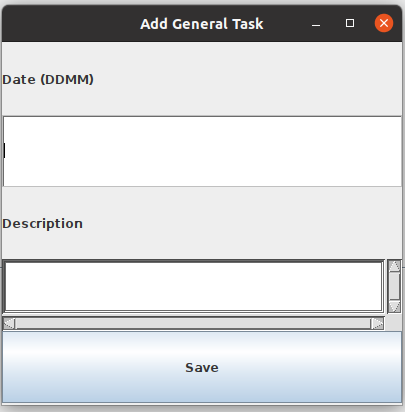
\includegraphics[scale=0.6]{images/add_general_task_screen.png}
\caption{Pantalla que para añadir una tarea general a la aplicación}
\label{fig:add_general_task_screen}
\end{figure}

En el caso de las tareas ``específicas'' se mostrarían de manera análoga con la diferencia de que la tabla que las muestra es de 3 columnas (fecha, nombre y descripción).


\subsection{Screen scrapping}

Para poder realizar la comunicación con 3270, inicialmente se había considerado utilizar \textit{WS3270} para realizar la comunicación, pero resultaba demasiado tedioso y generaba varios problemas. Es por ello que finalmente se ha utilizado \textit{s3270}\footnote{\url{http://x3270.bgp.nu/s3270-man.html}}, una herramienta de \textit{screen-scrapping}\footnote{\url{https://x3270.miraheze.org/wiki/Screen_Scraping}} para Linux. \\
Las funciones utilizadas para trabajar con el \textit{scrapper} se han obtenido de la siguiente \href{https://vebqa.github.io/f3270/release/doxygen/S3270_8java_source.html}{página}.\\
Para el uso de esta herramienta en Java se han seguido las indicaciones de la memoria, ejecutando el comando de la siguiente manera:
\begin{lstlisting}
final String commandLine = String.format("%s -model %s-%d %s:%d", s3270Path
	, type.getType(), mode.getMode(), hostname, port);

s3270 = Runtime.getRuntime().exec(commandLine);
out = new PrintWriter(new OutputStreamWriter(s3270.getOutputStream()
	, "ISO-8859-1"));
in = new BufferedReader(new InputStreamReader(s3270.getInputStream()
	, "ISO-8859-1"));
\end{lstlisting}
Se ha seguido un patrón de diseño \textit{Singleton} para garantizar que solo se cree una única conexión con el \textit{Mainframe}, junto a métodos encargados de añadir tareas (tanto específicas como generales) y mostrarlas. Para ello, se escribe en \textit{scrapper} cada uno de los comandos necesarios para realizar las operaciones. Han aparecido una serie de problemas relacionadas con la inserción y lectura de texto, ya que, en ocasiones, el programa enviaba información al \textit{scrapper} antes que este procesara la operación anterior, lo que provocaba sobreescrituras en el buffer. Para solventar este problema, se han añadido retrasos utilizando el comando "Thread.sleep(X)".

\textbf{{\Huge Hola Tambo (y Chusé) esta parte ya es tuya bro. Lo siento.}}


\end{document}